\documentclass[conference]{IEEEtran}

% Packages
\usepackage[utf8]{inputenc}
\usepackage[english]{babel}
\usepackage{amsmath}
\usepackage{amsfonts}
\usepackage{amssymb}
\usepackage{amsthm}
\usepackage{pdfpages}
\usepackage{graphicx}
\usepackage{epstopdf}
\usepackage{listings}
\usepackage{cite}
\usepackage{enumerate}
\usepackage{scientific}
\usepackage[colorlinks=false]{hyperref}
\usepackage{bookmark}

\usepackage[]{mcode}	%Matlab Code
\usepackage{tikz,pgfplots}	%Tikz
\usepackage{paralist}	% Auzählungen

% Bookmark Setup
\bookmarksetup{numbered}

% PDF Setup
\hypersetup{pdftitle={Assignment 2}, pdfsubject={Documentation of 2nd Homework}, pdfauthor={Stefan Röhrl}, pdfkeywords={MLIR Assignment 2}, pdfcreator={LaTeX}, hidelinks}


\begin{document}
%
% cite all references
%\nocite{*}
%
% paper title
% can use linebreaks \\ within to get better formatting as desired
\title{MACHINE LEARNING IN ROBOTICS\\ Assignment 2}

\author{\IEEEauthorblockN{Stefan Röhrl}
\IEEEauthorblockA{Technische Universität München, Arcisstraße 21, Munich, Germany\\
Email: stefan.roehrl@tum.de}}

% use for special paper notices
%\IEEEspecialpapernotice{(Invited Paper)}

% make the title area
\maketitle

\IEEEpeerreviewmaketitle

\section{Exercise}

\begin{flushleft}
Learned parameters for GMM after Expectation-Maximization.\\

Covariance Matrices:
$$
\Sigma_1 =
 \begin{pmatrix}
    3.946e-04 & 2.169e-04\\
	2.169e-04 & 1.277e-04
 \end{pmatrix}
$$

$$
\Sigma_2 =
 \begin{pmatrix}
    7.436e-04 & -5.914e-04\\
	-5.914e-04 & 6.098e-04
 \end{pmatrix}
$$

$$
\Sigma_3 =
 \begin{pmatrix}
	1.083e-03 & -4.244e-04\\
	-4.244e-04 & 2.431e-04
 \end{pmatrix}
$$

$$
\Sigma_4 =
 \begin{pmatrix}
	1.748e-04 & 2.616e-04\\
	2.616e-04 & 3.976e-04
 \end{pmatrix}
$$
\\
Means:
$$
\mu_1 =
 \begin{pmatrix}
	-1.470e-02 \\ -7.963e-02
 \end{pmatrix}
$$

$$
\mu_2 =
 \begin{pmatrix}
	-1.937e-02 \\ -1.664e-02
 \end{pmatrix}
$$

$$
\mu_3 =
 \begin{pmatrix}
	2.619e-02 \\ 6.173e-02
 \end{pmatrix}
$$

$$
\mu_4 =
 \begin{pmatrix}
	-4.319e-02 \\ 4.459e-02
 \end{pmatrix}
$$
Priors:
$$ \pi_1 = \begin{pmatrix} 2.012e-01 \end{pmatrix} $$

$$ \pi_1 = \begin{pmatrix} 2.971e-01 \end{pmatrix} $$

$$ \pi_1 = \begin{pmatrix} 2.617e-01 \end{pmatrix} $$

$$ \pi_1 = \begin{pmatrix} 2.400e-01 \end{pmatrix} $$
\end{flushleft}

\begin{figure}[h!]
  	\centering
    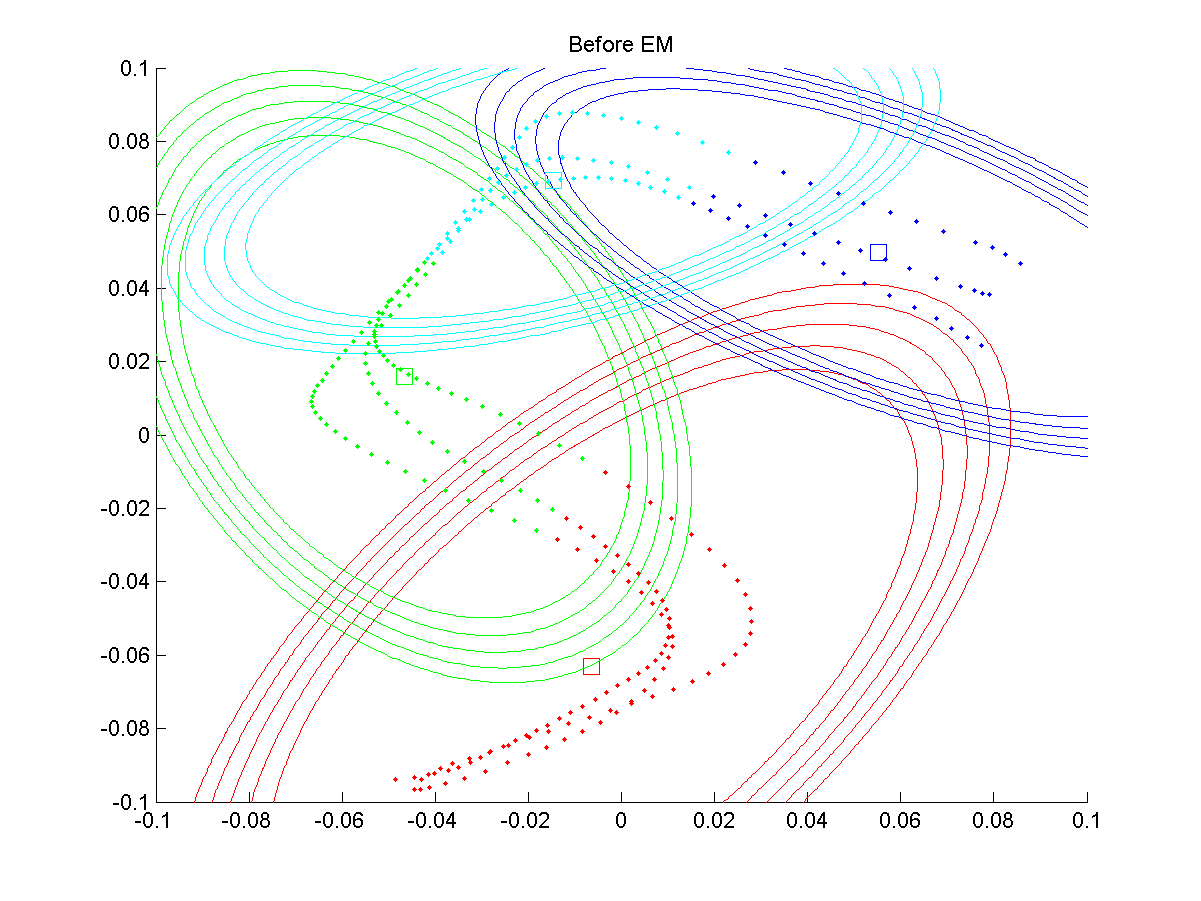
\includegraphics[width=0.5\textwidth]{img/1before_em.png}
    \caption{Gaussians and clusters before EM}
    \label{fig:before_em}
\end{figure}
The log-likelihood before the EM is: 1.353e+03

\begin{figure}[h!]
  	\centering
    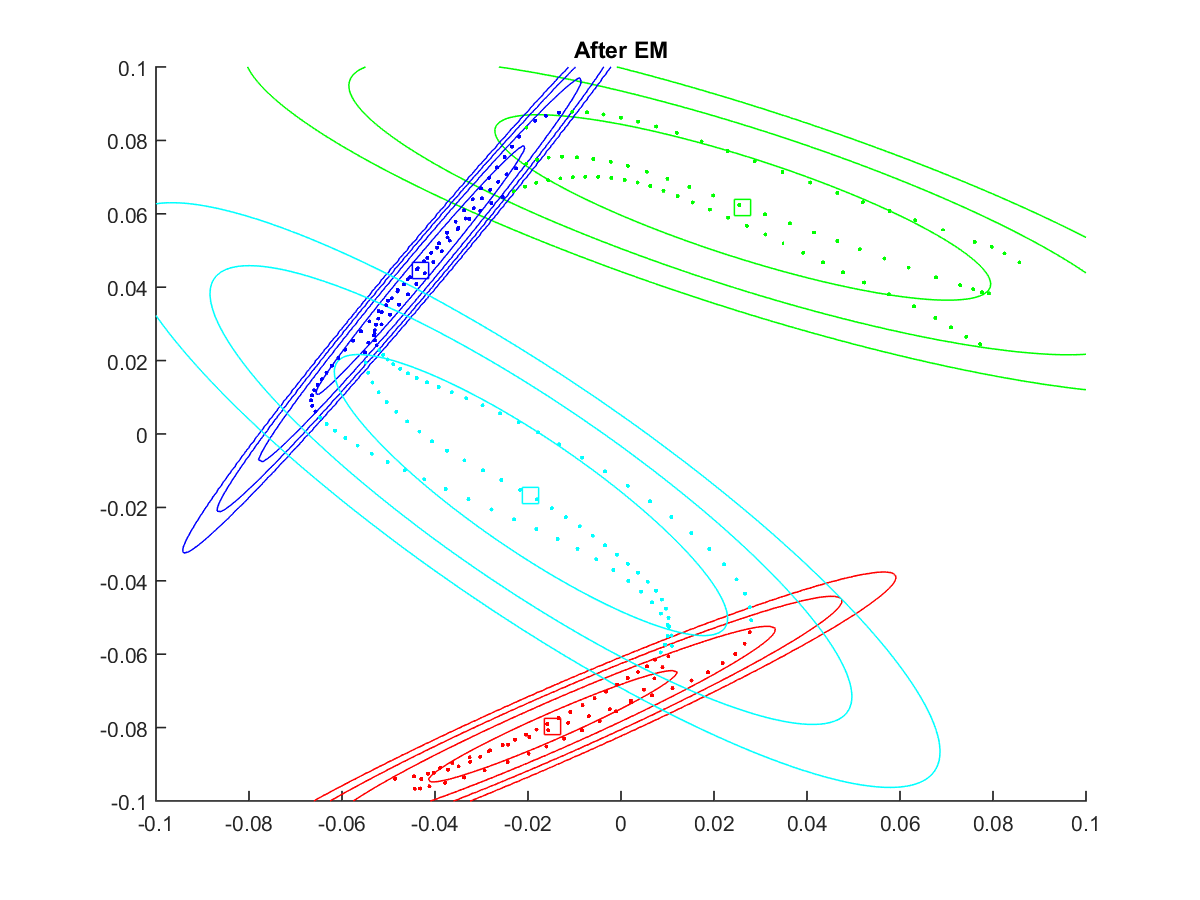
\includegraphics[width=0.5\textwidth]{img/1after_em.png}
    \caption{Gaussians and clusters after EM}
    \label{fig:after_em}
\end{figure}

The log-likelihood after the EM is: 1.448e+03
\newpage
~
\newpage
\section{Exercise}
The following list contains the log-likelihood and the labels of the Train Set. By labeling 1 stands for class \textit{train} and 0 stands for class \textit{test}.
$$
[log-likelihood, label] =
 \begin{smallmatrix}
 %logLH  & class\\
 &-2.312 &1.000\\
 &-2.312 &1.000\\
 &-14.620 &1.000\\
 &-24.359 &1.000\\
 &-46.196 &1.000\\
 &-46.196 &1.000\\
 &-70.710 &1.000\\
 &-87.584 &1.000\\
 &-68.024 &1.000\\
 &-67.401 &1.000\\
 &-89.607 &1.000\\
 &-92.499 &1.000\\
 &-126.337 &0.000\\
 &-115.001 &1.000\\
 &-70.706 &1.000\\
 &-94.465 &1.000\\
 &-115.794 &1.000\\
 &-95.986 &1.000\\
 &-117.905 &1.000\\
 &-81.088 &1.000\\
 &-89.167 &1.000\\
 &-89.331 &1.000\\
 &-50.709 &1.000\\
 &-80.423 &1.000\\
 &-57.664 &1.000\\
 &-40.420 &1.000\\
 &-56.434 &1.000\\
 &-45.929 &1.000\\
 &-45.789 &1.000\\
 &-39.312 &1.000\\
 &-39.312 &1.000\\
 &-39.172 &1.000\\
 &-38.899 &1.000\\
 &-38.348 &1.000\\
 &-38.348 &1.000\\
 &-38.070 &1.000\\
 &-37.936 &1.000\\
 &-37.803 &1.000\\
 &-37.803 &1.000\\
 &-37.669 &1.000\\
 &-37.193 &1.000\\
 &-36.850 &1.000\\
 &-36.583 &1.000\\
 &-36.449 &1.000\\
 &-35.973 &1.000\\
 &-35.630 &1.000\\
 &-35.630 &1.000\\
 &-35.287 &1.000\\
 &-35.287 &1.000\\
 &-34.944 &1.000\\
 &-34.601 &1.000\\
 &-34.258 &1.000\\
 &-34.258 &1.000\\
 &-24.866 &1.000\\
 &-24.866 &1.000\\
 &-24.866 &1.000\\
 &-2.312 &1.000\\
 &-2.312 &1.000\\
 &-2.312 &1.000\\
 &-2.312 &1.000
 \end{smallmatrix}
$$
\newpage
This list contains the log-likelihood of the Test Set. Where again 1 stands for class \textit{train} and 0 stands for class \textit{test}. As the result shows all test have a log-likelihood value over -120. Therefore all are classified as \textit{train}.
$$
[log-likelihood, label] =
 \begin{smallmatrix}
 %logLH  & class\\
 &-24.866 &1.000\\
 &-24.866 &1.000\\
 &-24.866 &1.000\\
 &-24.866 &1.000\\
 &-24.866 &1.000\\
 &-2.312 &1.000\\
 &-2.312 &1.000\\
 &-2.312 &1.000\\
 &-2.312 &1.000\\
 &-25.627 &1.000\\
 &-22.780 &1.000\\
 &-3.707 &1.000\\
 &-3.955 &1.000\\
 &-3.955 &1.000\\
 &-13.694 &1.000\\
 &-13.694 &1.000\\
 &-25.424 &1.000\\
 &-25.424 &1.000\\
 &-25.424 &1.000\\
 &-25.424 &1.000\\
 &-25.424 &1.000\\
 &-25.424 &1.000\\
 &-46.493 &1.000\\
 &-46.493 &1.000\\
 &-25.055 &1.000\\
 &-47.394 &1.000\\
 &-47.109 &1.000\\
 &-81.300 &1.000\\
 &-86.778 &1.000\\
 &-88.363 &1.000\\
 &-67.047 &1.000\\
 &-39.591 &1.000\\
 &-39.591 &1.000\\
 &-39.591 &1.000\\
 &-39.591 &1.000\\
 &-39.591 &1.000\\
 &-39.591 &1.000\\
 &-39.591 &1.000\\
 &-87.250 &1.000\\
 &-97.489 &1.000\\
 &-97.489 &1.000\\
 &-97.489 &1.000\\
 &-112.441 &1.000\\
 &-119.645 &1.000\\
 &-111.566 &1.000\\
 &-95.408 &1.000\\
 &-118.771 &1.000\\
 &-71.210 &1.000\\
 &-71.210 &1.000\\
 &-71.210 &1.000\\
 &-25.774 &1.000\\
 &-25.774 &1.000\\
 &-25.774 &1.000\\
 &-25.774 &1.000\\
 &-25.774 &1.000\\
 &-25.774 &1.000\\
 &-25.774 &1.000\\
 &-25.774 &1.000\\
 &-25.774 &1.000\\
 &-25.774 &1.000
 \end{smallmatrix}
$$
\newpage
\section{Exercise}
\begin{itemize}

\item \textbf{Policy Iteration:}

Reward Matrix
$$
R =
 \begin{pmatrix}
 &0.000 &0.000 &0.000 &0.000\\
 &0.000 &1.000 &-10.000 &-5.000\\
 &0.000 &0.000 &-10.000 &-5.000\\
 &0.000 &0.000 &0.000 &0.000\\
 &-10.000 &-5.000 &0.000 &1.000\\
 &0.000 &0.000 &0.000 &0.000\\
 &0.000 &0.000 &0.000 &0.000\\
 &-10.000 &5.000 &0.000 &0.000\\
 &-10.000 &-5.000 &0.000 &0.000\\
 &0.000 &0.000 &0.000 &0.000\\
 &0.000 &0.000 &0.000 &0.000\\
 &-10.000 &5.000 &0.000 &0.000\\
 &0.000 &0.000 &0.000 &0.000\\
 &0.000 &0.000 &-10.000 &5.000\\
 &0.000 &0.000 &-10.000 &5.000\\
 &0.000 &0.000 &0.000 &0.000
 \end{pmatrix}
$$

Used Value of $\gamma$: The used discount factor is held similar to the exercise 6 close to 1. Values from 0.99 to 0.999 were used.  \\

Iterations required: Depending on the random start values the algorithm need 5-9 Iterations till convergence.\\

\textit{To have a better surveillance over the states which were passed I modified the walkshow function in a way that the state number is printed under the image.}\\

Results of \textit{WalkPolicyIteration(s)}:

\begin{figure}[h!]
  	\centering
    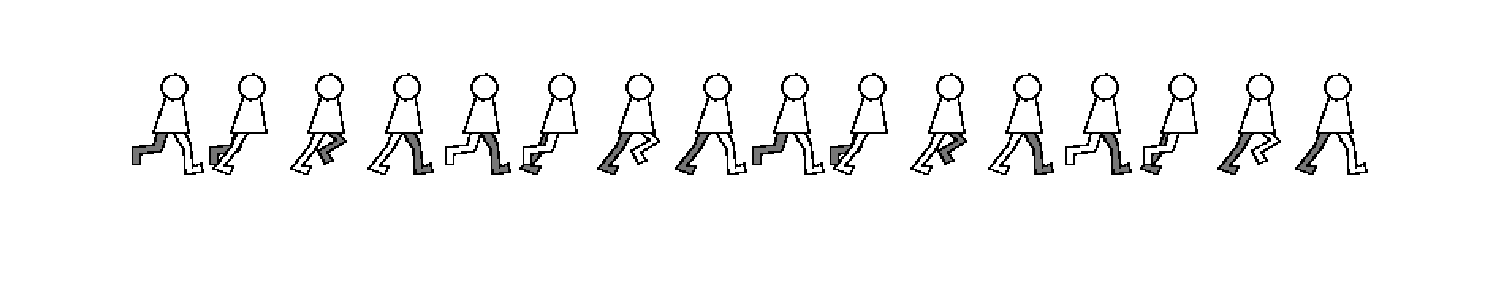
\includegraphics[width=0.5\textwidth]{img/3walkshow8.png}
    \caption{Results from starting state s = 8}
    \label{fig:3walkshow8}
\end{figure}

\begin{figure}[h!]
  	\centering
    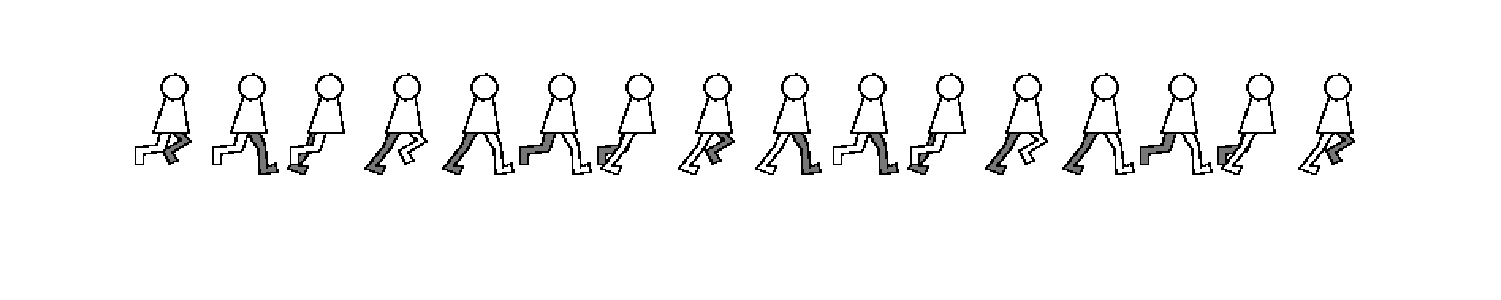
\includegraphics[width=0.5\textwidth]{img/3walkshow10.png}
    \caption{Results from starting state s = 10}
    \label{fig:3walkshow10}
\end{figure}

\begin{figure}[h!]
  	\centering
    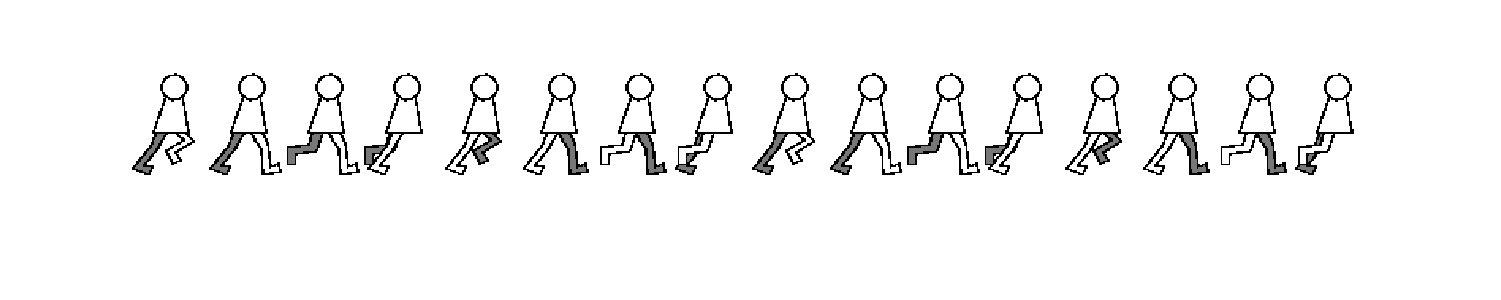
\includegraphics[width=0.5\textwidth]{img/3walkshow3.png}
    \caption{Results from starting state s = 3}
    \label{fig:3walkshow3}
\end{figure}

\item \textbf{Q-Learning:}\\
Used $\epsilon$: As the task says the probability $\epsilon$ should be small values between 0.1 and 0.2 are used. These values are static and don't change during the procedure. I am not sure if i found the ideal policy, but i think to improve the algorithm one should at first keep $\epsilon$ small to achieve fast convergence. After some steps when the algorithm has found a good policy one could increase $\epsilon$ to let the robot try more random actions. This should help to get out of local convergence to global convergence. I think the optimal policy could be found more often with this adaption, but as I can not prove the optimal policy I can not test my assumption.\\
\\
Used $\alpha$: A small value of 0.1 for $\alpha$ is used. This small learning rate promises a slow but good convergence. If $\alpha$ is choosen to big the convergence is not guaranteed. In contrast to this a small $\alpha$ needs much more steps because the convergence is very slow. Therefore 5000 iterations steps are used in \textit{WalkQLearning}. \\
\\
Outcomes of changing $\epsilon$ or using pure greedy policy: If one uses a too high value or too low value of $\epsilon$ it may be that the robot only walks with one leg or does other things which are not desired. It may randomly find a better policy than with mostly greedy steps but in general my tries have shown that values over 0.4 lead to a worse behavior. A pure random policy leads in many cases to a loop of actions and states. A pure greedy policy may also generate a loop, but also actions which are not desired. Against all odds the outcomes are not always the same for the same start state. However these pure greedy out comes are not always desired. Behaviors as mentioned above like the walking with only one leg may occur. One could improve that by choosing another reward matrix and lead the robot to the right cycle, but this would not be learning any more. Therefore it is important to choose a proper $\epsilon$. It must be small enough to choose the actions which will get the most reward to learn the waling. It also must allow random steps so that the algorithm is not stuck in local convergence.\\

Steps needed: I only can assume the number of steps which are nescessary to find the optimal policy as i am not able to classify the optimal policy. I used 5000 iterations to achieve good results. 500 steps are to few to find a good policy with the small learning rate $\alpha$ which was used. I also did not see any improvement in increasing the steps over 5000. \\

\newpage
Results of \textit{WalkQLearning(s)}: 
\\
\\
\textit{As one starts with a random initialisation and a partly random $\epsilon$-greedy policy the results are not always the same in every try. here are the best results the algorithm delivered. The plots were generated with $\alpha=0.1$, $\gamma=0.999$, $\epsilon=0.1$, $Steps=5000$}

\begin{figure}[h!]
  	\centering
    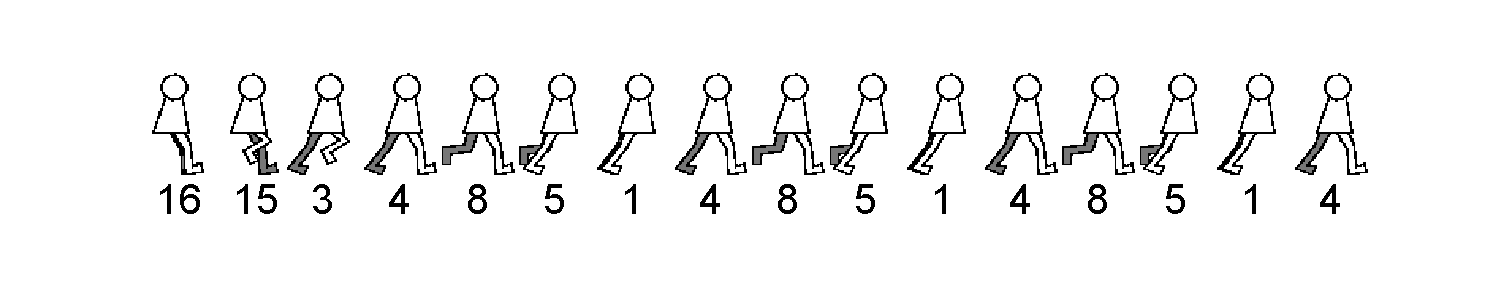
\includegraphics[width=0.5\textwidth]{img/3walkshow16.png}
    \caption{Results from starting state s = 16}
    \label{fig:3walkshow16}
\end{figure}

\begin{figure}[h!]
  	\centering
    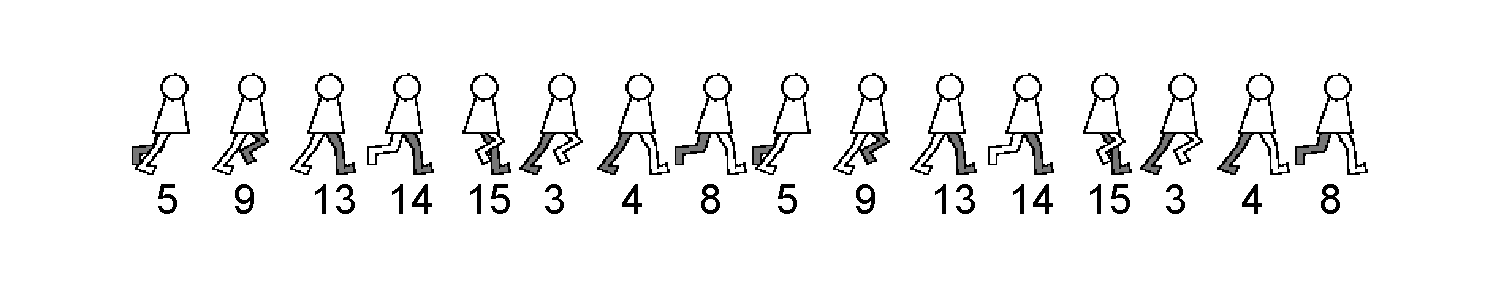
\includegraphics[width=0.5\textwidth]{img/3walkshow5.png}
    \caption{Results from starting state s = 5}
    \label{fig:3walkshow5}
\end{figure}

\begin{figure}[h!]
  	\centering
    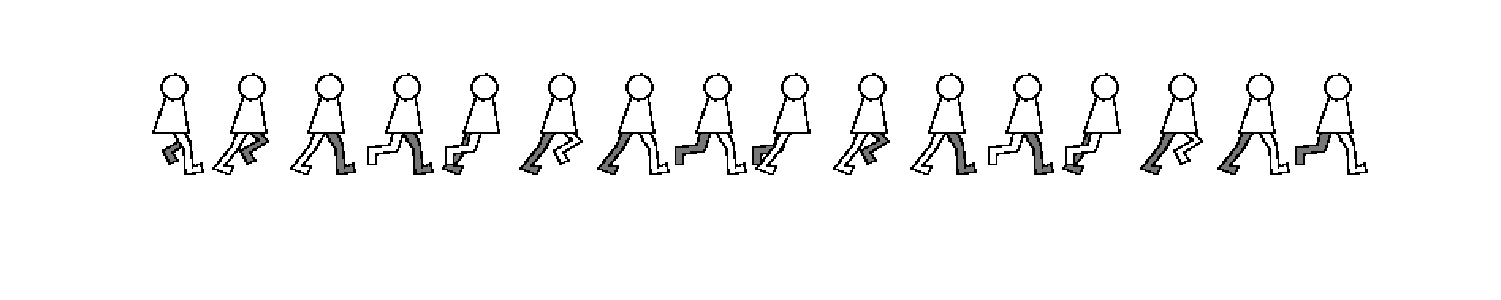
\includegraphics[width=0.5\textwidth]{img/3walkshow12.png}
    \caption{Results from starting state s = 12}
    \label{fig:3walkshow12}
\end{figure}


\end{itemize}
\end{document}


